%% Copernicus Publications Manuscript Preparation Template for LaTeX Submissions
%% ---------------------------------
%% This template should be used for copernicus.cls
%% The class file and some style files are bundled in the Copernicus Latex Package, which can be downloaded from the different journal webpages.
%% For further assistance please contact Copernicus Publications at: production@copernicus.org
%% https://publications.copernicus.org/for_authors/manuscript_preparation.html


%% Please use the following documentclass and journal abbreviations for discussion papers and final revised papers.


%% 2-column papers and discussion papers
%\documentclass[acp, manuscript]{copernicus}
\documentclass[acp]{copernicus} % final format

%% \usepackage commands included in the copernicus.cls:
%\usepackage[german, english]{babel}
%\usepackage{tabularx}
%\usepackage{cancel}
%\usepackage{multirow}
%\usepackage{supertabular}
%\usepackage{algorithmic}
%\usepackage{algorithm}
%\usepackage{amsthm}
%\usepackage{float}
%\usepackage{subfig}
%\usepackage{rotating}


\begin{document}

\title{Wavelength calibration of Brewer spectrophotometer using a tuneable pulsed laser and implications to the Brewer ozone retrieval}


% \Author[affil]{given_name}{surname}
\Author[1,2]{Alberto}{Redondas}
\Author[3]{Saulius}{Nevas}
\Author[4,2]{Alberto} {Berjón}
\Author[3]{Meelis-Mait} {Sildoja}
\Author[1,2]{Sergio F.}{León-Luis}
%\author[6]{Omar el Gawhary} 
%\author[7]{Ilias Fountoulakis}


\affil[1]{Agencia Estatal de Meteorología, Izaña Atmospheric Research Center, Spain}
\affil[2]{Regional Brewer Calibration Center for Europe, Izaña Atmospheric Research Center, Tenerife, Spain}
\affil[3]{Physikalisch-Technische Bundesanstalt (PTB), Braunschweig, Germany}
\affil[4]{University of La Laguna, Department of Industrial Engineering, S.C. de Tenerife, Spain}





\runningtitle{Brewer Wavelength Calibration}

\runningauthor{Redondas}

\correspondence{Alberto Redondas (aredondasm@aemet.es)}



\received{}
\pubdiscuss{} %% only important for two-stage journals
\revised{}
\accepted{}
\published{}

%% These dates will be inserted by Copernicus Publications during the typesetting process.


\firstpage{1}

\maketitle



\begin{abstract}

In this contribution we present the wavelength calibration of the traveling reference Brewer of the Regional Brewer Calibration Center (RBCC-E)  at PTB in Braunschweig, Germany. The wavelength calibration is needed for the calculation of the ozone absorption coefficients used by the Brewer ozone algorithm. In order to validate the standard procedure for determining Brewer’s wavelength scale, a calibration has been performed by using a tuneable laser source at PTB in the framework of the EMRP project ENV59 ATMOZ "Traceability for the total column ozone". Here we compare these results to those of the standard procedure for the wavelength calibration of the Brewer instrument. Such a comparison allows validating the standard methodology used for measuring the ozone absorption coefficient with respect to several assumptions. The results of the laser-based calibrations reproduces those obtained by the standard operational methodology and shows that there is a underestimation of 0.8\%  due the use of the parametrized slit functions. 
\end{abstract}

\copyrightstatement{TEXT}

\section{Background}

The wavelength calibration is needed for calculation of the ozone absorption coefficient used by the Brewer ozone retrieval algorithm. The Brewer spectrophotometer has two operating  modes. In the ozone mode, used for the total ozone column measurements, the diffraction grating stays at a fixed position while the six operational wavelengths are selected by a rotating slit mask.  The scanning mode is used to perform spectral irradiance measurements in the ultraviolet (UV) spectral range. In this mode, the slits are fixed and the spectral scan is carried out by turning the diffraction grating. The usual wavelength calibration procedure is performed in the scanning mode by analyzing recorded emission lines of the spectral discharge lamps, which are usually mercury (Hg), cadmium (Cd) , and zinc (Zn). Using the spectral lines provided in Table \ref{tab:dsp_lines} allows determining the central wavelengths and the corresponding FWHM (full width at half maximum) of the slit functions as well as the relation between the positions of the grating  and the corresponding instrument wavelengths (dispersion relation) required to determine the operational wavelengths used for the ozone determination. To obtain the ozone absorption coefficients, the instrumental slit functions are convoluted whit the Bass \& Paur ozone absorption cross-section data.
The use of the of the tuneable laser  source allow us to:
\begin{itemize}

    \item Calculate the ozone absorption coefficients directly in the ozone mode. The normal ozone absorption coefficient determination uses the scan of the spectral lines in the scanning mode so that a dispersion relation is used to convert grating positions in micrometer steps to wavelengths assuming a quadratic relation. Scanning directly with the laser around the ozone operational wavelengths in the ozone mode we can determine the instrumental slit functions directly and weight them with the ozone absorption cross-sections without need for the assumptions of the slit functions and the dispersion relations used in the normal operational procedure.
    \item Calculate the dispersion relation based on regularly spaced reference spectral lines provided by the tuneable laser instead of the irregularly distributed  emission lines of the  Hg, Cd and Zn spectral lamps. 
\end{itemize}

%The objective of this work is  to validate the standard procedure for the brewer spectrophotometer, For that we compare  to do that we perform 3 experiments, the standard procedure described on secion 2, the experiments results obtained with the laser , using the brewer on ozone mode (the lases scans ) and finally using the laser

During the experiment we performed three measurements: 
\begin{enumerate}


\item The standard method for the dispersion measurements using spectral lamps described in secion 2.

\item  Direct dispersion measurements (laser scanning). 
While Brewer is measuring in ozone mode and in aerosol mode, the laser wavelength is sweeped ±2\unit{nm} with a step of 0.05\unit{nm} around the six Brewer operational wavelengths selected by the rotating slit mask for different grating positions.

%(ozone and aerosol). 


\item  Dispersion measurements using tuneable laser (Brewer scanning): while the laser is emitting at a fixed wavelength, the Brewer will scan ±2\unit{nm} around this wavelength in scanning mode by moving the grating and using the 6 slits. This Brewer scan is carried out at wavelengths ranging from 290 \unit{nm} to 365 $\unit{nm}$ with an increment of 5$\unit{nm}$.  The results allow us to estimate the dispersion approximation error due to the lack of spectral lines at the end of spectral range of the Brewer spectrophotometer and due to the fact that that the emission lines of the used lamps are not equally spaced.

%\item 
\end{enumerate}







\section{Calibration of the Brewer spectrophotometer}
\label{sec:calibration}


The Brewer instrument measures the irradiance of direct sunlight at six nominal wavelengths ($\lambda$) in the UV range (303.2, 306.3, 310.1, 313.5, 316.8, and 320.1~\unit{nm}), each spectral band covering a bandwidth of 0.5~\unit{nm} (resolution power $\lambda/\delta\lambda$ of around 600). The spectral resolution is achieved by a holographic grating in combination with a slit mask that selects the channel to be analyzed by a photomultiplier (PMT). The longest four wavelengths are used for the ozone calculation. Based on the Lambert-Beer law, the total ozone column in the Brewer algorithm can be expressed as:

\begin{equation}
	\label{eq:ozone}
	X = \frac{{F - ETC }}{\alpha  \mu }\
\end{equation}

where $F$ are the measured double ratios corrected for Rayleigh effects, $\alpha$ is the ozone absorption coefficient, $\mu$ is the ozone air mass factor, and $ETC$ is the extra-terrestrial constant. The $F$, $\alpha$ and $ETC$ parameters are weighted functions at the operational wavelengths with weighting coefficients $w$:
      
\begin{equation}	
	F = \sum\limits_i^4 {{w_i} {F_i} - \frac{p} {p_0} \beta_i \mu }
\end{equation}
      
\begin{equation}	
	\alpha = \sum\limits_i^4 {{w_i} {\alpha_i} }
\end{equation}

\begin{equation}	
	ETC = \sum\limits_i^4 {{w_i} {{F_0}_i} }
\end{equation}

where, $\beta_i$ are the Rayleigh coefficients,  $p$ is the climatological pressure at the measurement site, $p_0$ is the pressure at sea level, and $F_0$ are the individual extra-terrestrial constants at each wavelength. The weights $w=[1,-0.5,-2.2, 1.7]$ have been chosen so as to minimize the influence of SO$_2$ and verify:
      
\begin{equation}	
	\sum\limits_i^4 {{w_i} }=0
\end{equation}
     
\begin{equation}	
	\sum\limits_i^4 {{w_i} {{\lambda}_i} }=0
\end{equation}

This widely eliminates absorption features which depend, in local approximation, linearly on the wavelength, like for example the contribution from aerosols.

We can divide the calibration in three steps including instrumental calibration, wavelength calibration, and ETC transfer:

\begin{enumerate}
	\item The instrumental calibration includes all the parameters that affect the measured signal counts ($F$), in particular, photomultiplier dead time correction, temperature coefficients and filter attenuation.
	\item Wavelength calibration is needed to determine the ozone absorption coefficient. The so-called "dispersion test" is used to obtain the particular wavelengths for the instrument and the slits, or instrumental functions, of each spectrophotometer. Note that the precise wavelengths of every Brewer spectrophotometer are slightly different from instrument to instrument. 
	\item Finally, the ETC transfer is performed by comparison with the reference Brewer instrument or, in the case of the reference instruments, by the Langley method.
\end{enumerate}

%The calibration process can be considered as cycle changes. Instrumental and/or wavelength calibration will affect the final ETC and changes in the wavelength calibration will affect also to the final ETC. 

The Brewer wavelength calibration follows the operative procedure \citep{Grobner1998, kerr2002new} used by the Regional Brewer Calibration Center-Europe (RBCC-E) at the calibration campaigns. In summary, the individual wavelengths (bands) in the Brewer instrument are selected through the use of a stainless steel mask of seven slits located at the focal plane of the spectrometer. The particular wavelength is determined by analyzing the measurements of  a series of discharge lamps during so-caled dispersion test, which determines the central wavelength and FWHM of every slit. Then the  wavelength setting is optimized to minimize the effect of wavelength shift during the operation of the instrument by performing the so-called sun-scan test \citep{sun_scan_ios}. Finally, the ozone absorption coefficient is determined for every slit.   


The  ozone absorption coefficient is defined as:

\begin{equation}
\widetilde \alpha (X,\mu ) = \sum {{w_i}} \frac{{\int {\alpha (\lambda )*S(\lambda ,\lambda ')*} F(\lambda ,\lambda ',X,\mu )d\lambda '}}{{\int_{}^{} {S(\lambda ,\lambda ')*F(\lambda ,\lambda ',X,\mu )d\lambda '} }}
\end{equation}

Where $S$ is the instrumental slit function for the corresponding wavelength, $F$is the sun spectrum that depends mostly on the ozone concentration and airmass, and $\sigma$ is the ozone cross-section at the temperature of $-$46.3\, \unit{\degree C} for Dobson 
and at $-$45\, \unit{\degree C} for Brewer instruments. 

The Brewer operative method uses the following assumptions:
\begin{enumerate}
	\item Use  “ideal” slits; the slit functions are parametrized as trapezoids, i.e., isosceles triangles truncated at 0.82 height.
	\item Stray light is not considered, i.e., zero slit function values are assumed outside the triangle. 
	\item The FWHM of the triangle is dependent of the slit and it is derived from the dispersion test.
	\item The ozone cross sections are expressed by the Bass \& Paur absorption coefficient data set.
 	\item Solar spectrum is not considered ,  ($F$==1)
\end{enumerate}

Under these assumptions, the ozone effective absorption is essentially obtained the same way as in the approximation method of \citet{Bernhard2005} used with Dobson spectrophotometers. (see Eq.~\ref{eq:conv}).


      \begin{equation}
      \label{eq:conv}
            %\alpha_i = {{\int {\sigma(\lambda)\, {S_i}(\lambda)\, \text{d}\lambda } }
            %\over{\int_{}^{} {{S_i}(\lambda )\text{d}\lambda } }}
            \alpha_i = \frac{\int \sigma(\lambda) S_i(\lambda) \mbox{d}\lambda}{\int S_i(\lambda) \mbox{d}\lambda}
      \end{equation}


\subsection{Dispersion Test}

The Brewer spectrophotometer is constructed based either on single or double monochromatoror of modified Ebert–Fastie type, generally referered to as single or double Brewer, respectively. The first monochromator disperses the incoming radiation onto six exit slits. In the case of the double Brewer , the six exit slits  (intermediate slits) of the first monochromator are the entrance slits to a second monochromator that is used in subtractive mode. The wavelength is selected by choosing one of the six exit slit (ozone mode) or rotating the grating (scanning mode). The rotation of the grating is managed by a drive mechanism consisting of a motor-driven micrometer linked to an arm that rotates the grating. The smallest wavelength increment corresponding to one stepper motor step varies steadily from approximately 8.0 pm to 7.0 pm ( 0.0080 \unit{nm} ). 

The dispersion relation, which provides the  relation between the micrometer steps and monochromator set wavelengths, is determined by scanning the emission lines as described in section 1. The line scans are carried out with with an increment of 10 motor steps (~0.6A). From the results, the central position and the FWHM of the slit function are calculated in  motor steps assuming an isosceles triangle. The both sides of the peak are  fitted to a straight line taking only the function values above 20\%  and bellow 80\% of the normalized peak. The central point is calculated by the intersection point and the FWHM is the with of the triangle. (Figure x). Finally, the dispersion relation is calculated using a quadratic polynomial or the cubic approximation \citep{Grobner1998}. This relation is used to transform the previously determined central positions and FWHMs of the slit functions in micromenter steps to a wavelength scale.


% mercury test
   The stability of the wavelength calibration during Brewer operations is checked by measuring the internal Hg lamp. In most of the Brewers, the 302 \unit{nm} double line (302.150 nm and 302.347 nm) is used due to its proximity to the Brewer operational wavelengths. However, for Brewer \#185 and for an increasing number of other Brewer the test is  performed using the more powerfull 296.7 \unit{nm} line. The wavelength test includes 12 measurements of the line from the mercury lamp on slit 0, 10 steps of the micrometer motor apart. The obtained curve for the line peak is compared to a stored reference one. The comparison is done by shifting the two scaned curves against each other and calculating the correlation coefficient between the two after each shift. The interpolated step number yielding the maximum of the correlation coefficient provides the reference micrometer position.(\citep{savastiouk2005improvements}). If the required adjustment of the micrometer position is more than one and a half motor steps, the test is repeated. The accuracy of the wavelength setting of the Brewer instrument achieved by such an approach is limited by one and half motor steps and cannot be better than about 0.86A. This affects the ozone abortion coefficient by approximately of 0.10 \unit{atm cm^-1} and the ozone concentration by 0.3\%.
   % the error of a step funciotn of  1.5 step wide =   1.5 / sqrt(3)  is 0.86
  


\subsection{Sun scan}
\citet{savastiouk2005improvements} 


\section{ Pulsed laser-based measurements}

\subsection{Instrumental setup}

For scanning the bandpass functions of the Brewer instrument, an upgraded PLACOS setup \citet{Nevas2009} featuring a tuneable pulsed laser system based on an Optical Parametric Oscillator (OPO) was used at Physikalisch-Technische Bundesanstalt (PTB) in Braunschweig  (Figure \ref{fig:opo}). The new OPO system generates 3-6 ns pulses at 1 kHz repetition rate in the spectral range from 210 \unit{nm} to 2600 \unit{nm}. The laser wavelengths were monitored during the measurements by a wavemeter (laser spectrum analyzer) and a high-resolution spectrometer with an uncertainty of 0.01 nm. The laser beam was guided into the direct port of the Brewer spectrophotometer. A fraction of the beam was directed to a monitor photodiode in order to account for the ouput power changes of the laser beam. The photocurrent of the silicon photodiode was measured by a charge meter.


% monitor description
% accuracy


In contrast with the standard calibration procedure, where the Brewer instrument scans the lines of the spectral lamps, in this experiment the Brewer measures in ozone mode. Here, the Brewer grating is fixed at the ozone position while the coupled laser beam is measured using the seven slits (slit  \#1 is used to obtain the dark signal values). During these measurements the wavelength of the OPO system is scanned with 0.01 \unit{nm} step. The experiment is complemented by the measurements in the Brewer scanning mode, where the tuneable laser is used as a source of spectral lines covering the range from 290\unit{nm} to 360 \unit{nm} on a regular grid with 5 \unit{nm} step.



\subsubsection{Non-linearity of the PMT }

The Brewer detector system, which is based on a photomultiplier tube (PMT), responds non-linearly to pulsed sources. For the measurements of pulsed sources, the PMT manual advises to change the electronics configuration. As the main objective was to validate the operational wavelength calibration of the Brewer, we decided to keep the instrument configuration equivalent to that during the field operations. The non-linearity problem was solved by determining the respective correction function. For this purpose, the power of the laser beam was varied while simultaneously measuring signals of the PMT and the linear monitor photodiode.


The ratios of the measured Brewer counts to the recorded monitor photodiode signals are shown in figure  \ref{fig:no}. The non-linearity is evident in the figure together with hysteresis region near $10^4$  Brewer counts/seconds. The correction is not reliable  around $10^3$ counts/seconds and lower than 100 counts/seconds. As we can control the power of the laser beam, it is possible to work on the “flat regions” of the non-linearity characteristics and apply the determined correction. This correction does not affect the calculated central wavelength of the slit functions, though, it does affect the determined FWHM values (Figure \ref{fig:slitcor}) if the correction is not applied.

The nonlinearity correction is not reliable for signals lower than 100 counts/seconds. Also we observed (Figure \ref{fig:laser_log}) that the recorder dark signal values (measurements performed with the blocked slit \#1) were highest immediately after exposing the PMT to the laser light. The dark signal of the PMT was then gradually fast decreasing with time after the excitation, which may cause the signal values obtained for slit \#1 (measured immediately after slit \#0) be higher than for the other slits measured afterwards.

\subsubsection{Slit parametrization }

The Brewer algorithms assume trapezoidal slits cut at 0.87 of the height (Figure \ref{fig:param}) with the  center wavelength and the FWHM calculated for every slit from the dispersion relation. The laser measurements allow us to estimate the effect on the ozone calculation if we use the directly measured slit functions instead of the parametrised ones. For this purpose we calculate the ozone absorption coefficients for the four ozone cross sections evaluated in the  "ACSO" comitee ("Absorption Cross Sections of Ozone") ( \citet{orphal2016absorption}.

Among the available data sets there are versions of Bass and Paur~(1985) cross-sections denoted as Brewer operational (Brw), IGACO quadratic coefficient (B\&P), the cross-sections of  Daumont Brion Malicet (DBM) (\citet{ daumont_ozone_1992}, \citet{brion_high-resolution_1993}, and \citet{malicet_ozone_1995} ), and the newly recommended data set for ozone ground-based calculation by Serdyuchenco, Groshelev, Weber (SGW) \citep{serdyuchenko_high_2012,gorshelev_high_2012,amt-9-4459-2016}. 


Using the measured slit functions, the calculated effective ozone cross sections are $~0.9\%$ higher compared to those obtained by using the parametrized Brewer slits in the standard procedure (Table \ref{tab:slit_param}) independently of the cross sections used.


\section{Comparison }

The experiment allows us to validate the Brewer standard methodology used to perform the wavelength calibration. For this purpose, we compare laser-based wavelength calibration results to those yielded by the standard operative method based on scanning the spectral lamps in case of both the quadratic and the cubic fit to the dispersion relation.

Figure \ref{fig:cw_comp} shows discrepancies between the central wavelengths calculated by the quadratic and the cubic fits to be bigger than 0.1 A for wavelength adove 320 \unit{nm} and much bigger near 350 nm. This is  also indicated by the systematic residuals of the quadratic fit that are much larger than for the cubic fit (see figures 9 and 10). This indicates that the quadratic fit is only valid in the ozone range (310-320 nm). The comparison of the calculated FWHMs (Figure \ref{fig:cw_comp} ) shows a different pattern with a difference of 0.1A between the direct and the scanning methods in the ozone range and with a smaller difference between the quadratic and the cubic fits.  

The differences to the directly calculated ozone absorption coefficients are summarized for the six measurements in table \ref{tab:o3abs_sum}, taking as a reference the direct measurements. The quadratic fits result in bigger differences of around 1\% whereas in the case of the cubic fits the differences decrease to 0.3\% and  0.1\%  when the laser or the discharge lamps are used, respectively.   




\conclusions{}

\begin{enumerate}

%\item 
 %We don't find significant differences when different input optics is used for the wavelength characterization, placing the spectral source on the global port, direct port or using the Hg internal lamp are interchangeable for this purposes.

    \item Using the measured slit functions instead of the paramterized ones increases the ozone absorption coefficients and consequently the calculated ozone values by 0.8\%.

    \item The quadratic dispersion relation fit used in the standard Brewer algorithm is not suitable outside the ozone range 310 nm - 320 nm. The residuals show a systematic pattern, which is particularly important in the higher range.%-> effect o the ozone<-

    \item The comparison of the results of the three experiments shows a maximum difference of 0.3\% if the cubic fit is used. The respective error in the ozone absorption coefficient obtained using direct measurement in ozone mode and operative discharge lamp method is only of 0.1\%. This confirms the standard procedure used for the RBCC-E calibrations.

\end{enumerate}




%% ONE-COLUMN FIGURES
\clearpage
%%f
\begin{figure}[t]
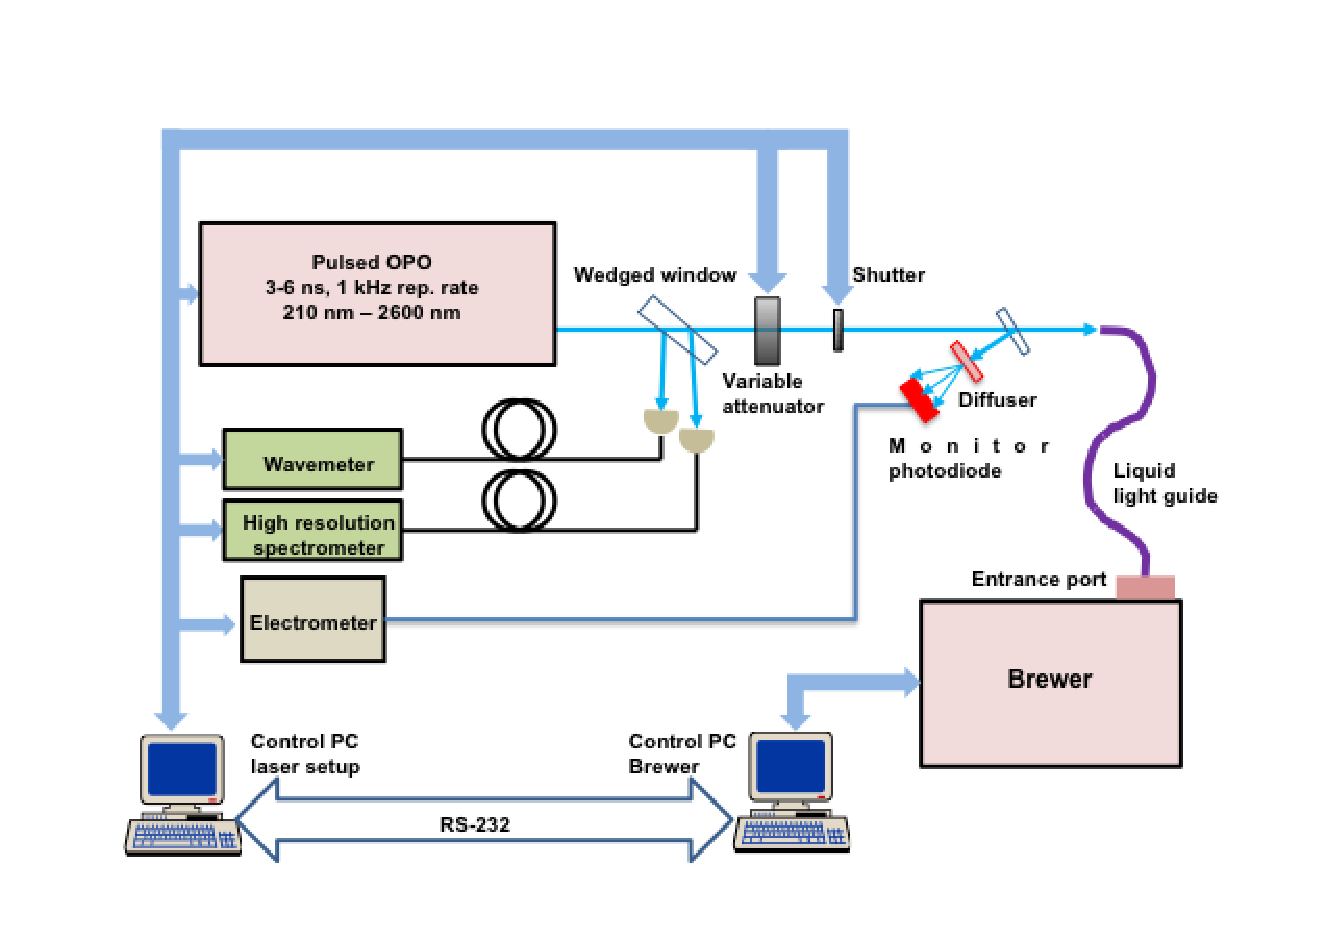
\includegraphics[width=8.3cm]{opo.eps}
\caption{Pulsed optical parametric oscilator (OPO)-based setup at PTB that was used for measuring the slit functions of the Brewer spectrophotometer.}
\label{fig:opo}
\end{figure}




\clearpage
%%f
\begin{figure}[t]
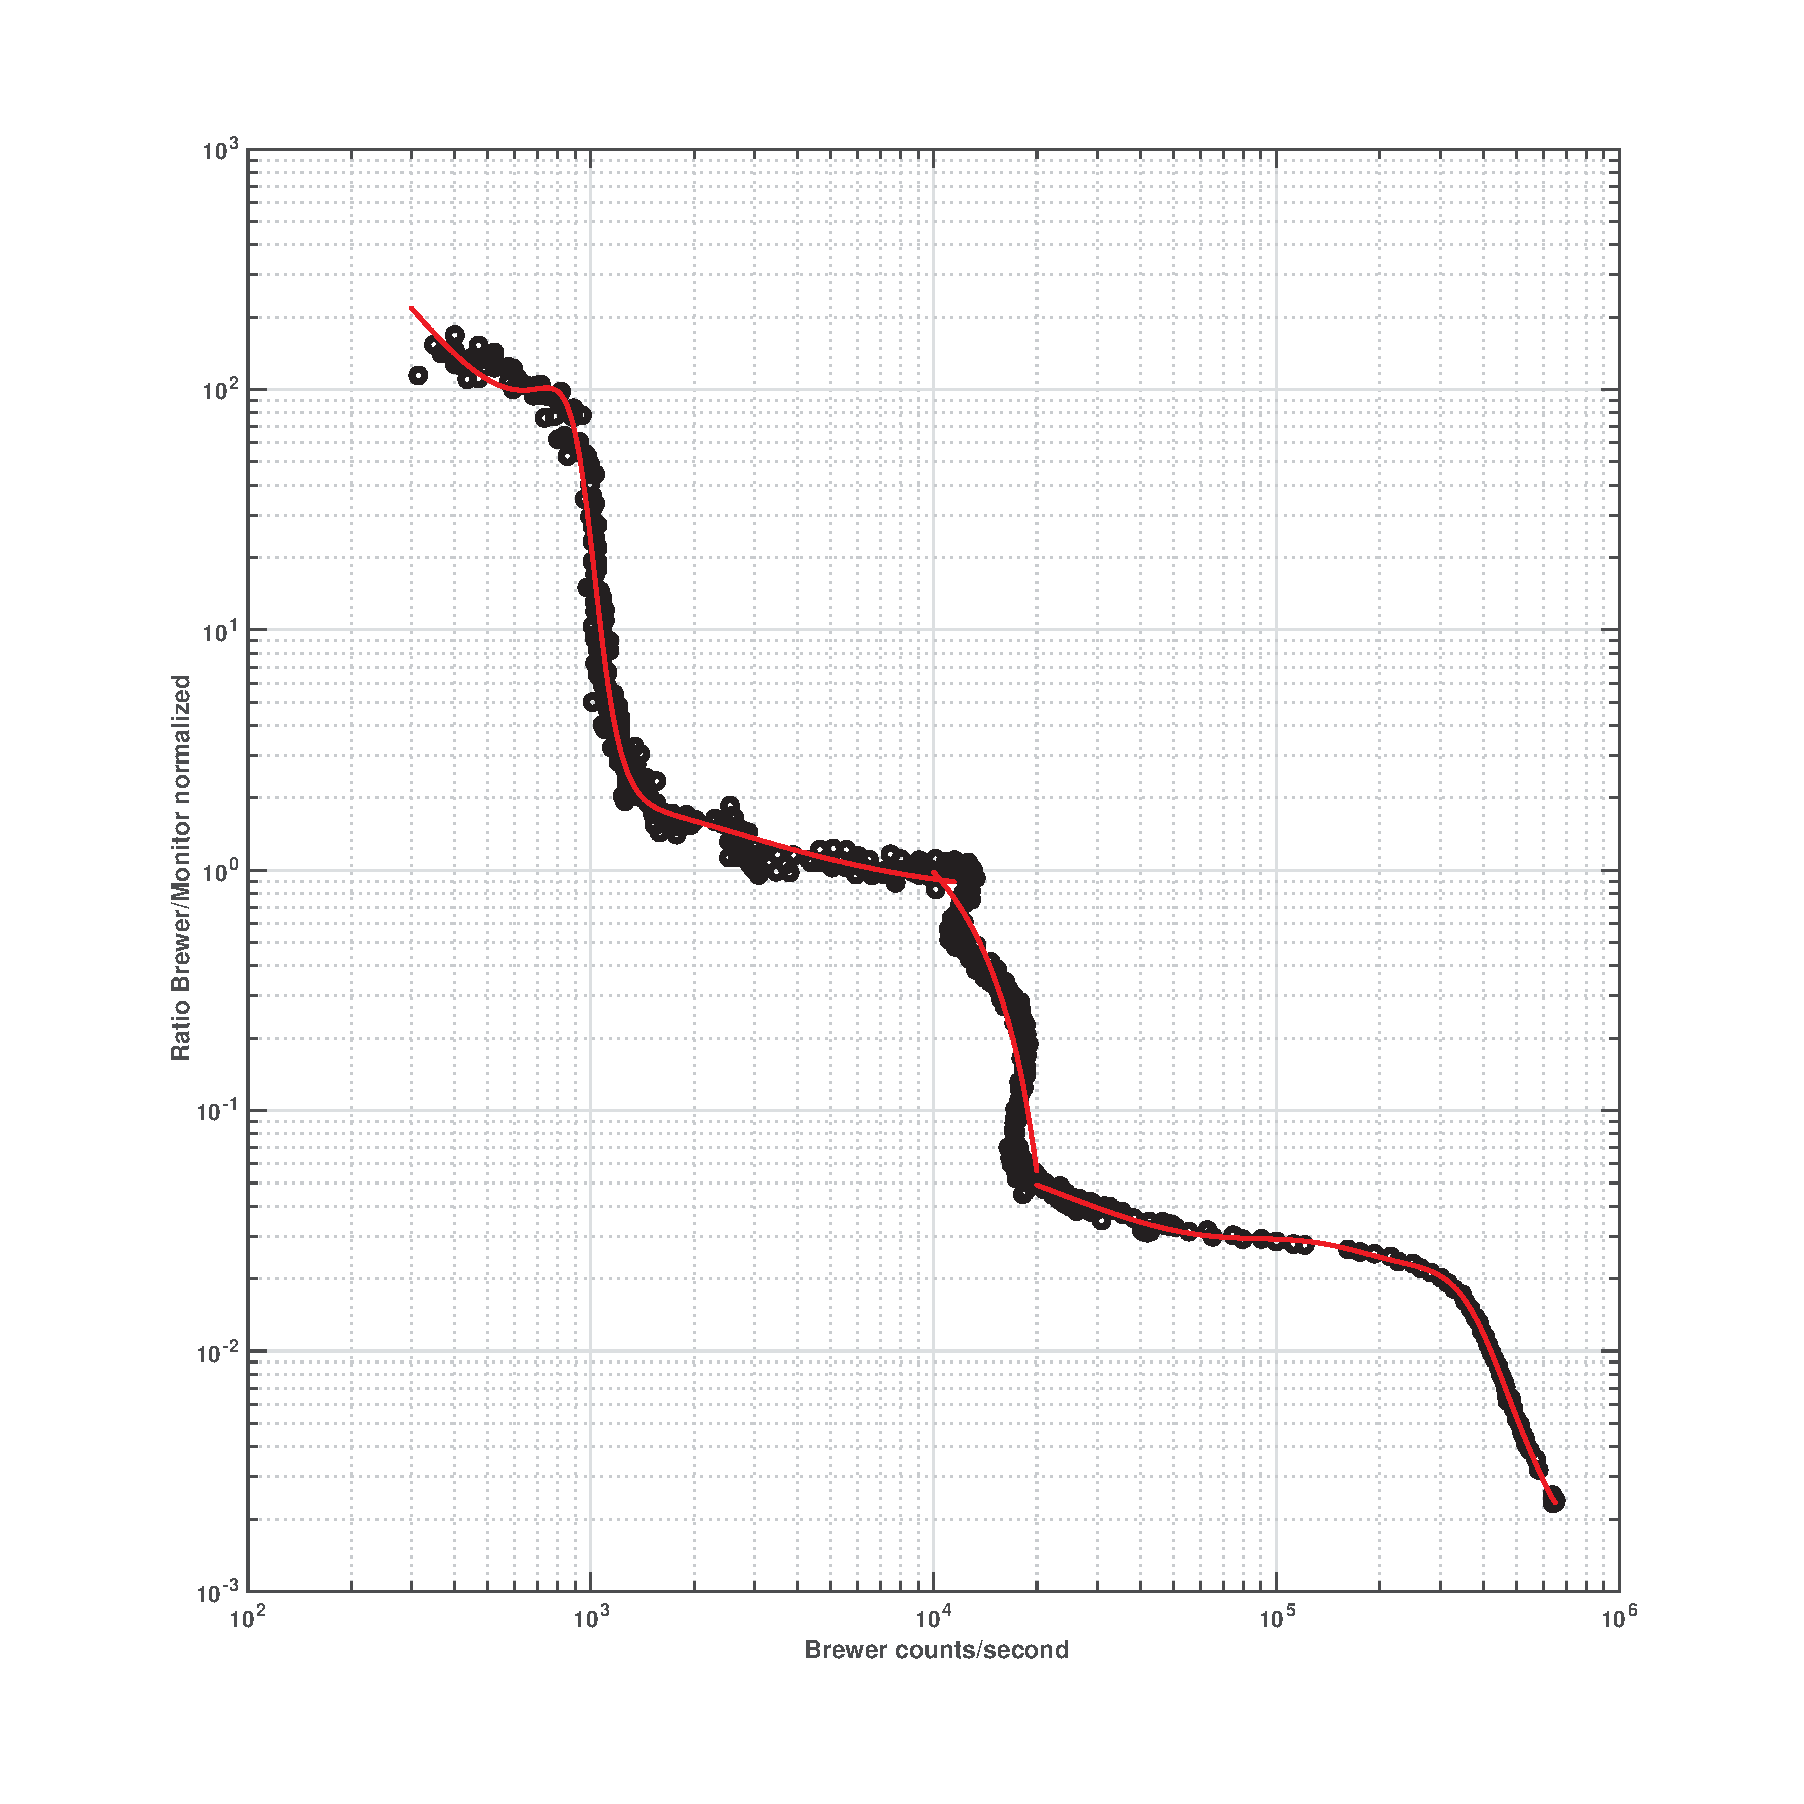
\includegraphics[width=8.3cm]{General_NoLinearity_corr.eps}
\caption{ Log-log plot of the normalized ratio of measured Brewer counts to the monitor photodiode signal, which is proportional to the laser power, plotted as a function of the Brewer counts/s. The black points shows the measured points while the red curve is the fit used to correct the Brewer signals for the nonlinearity.}
\label{fig:no}
\end{figure}
\clearpage
%%f
\begin{figure}[t]
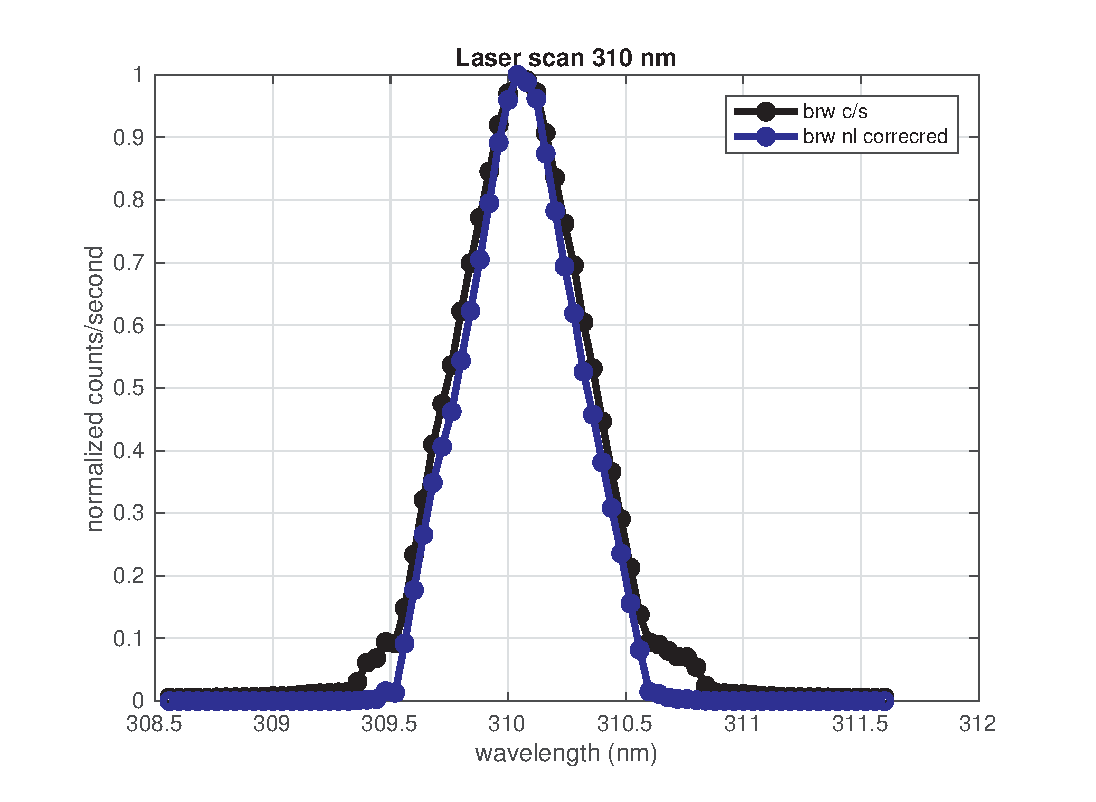
\includegraphics[width=8.3cm]{figures/General_Corrected_vs_uncorrected.eps}
\caption{Measured slit function of the 310 nm slit (slit \#4): uncorrected counts/second (black) and non-linearly-corrected values (dark blue). The central wavelength determination is not affected by the nonlinearity but the FWHM is bigger if the correction is not applied. The hysteresis is evident from the asymmetry of the function at the low values region of the plot. As the method uses the normalised values only between 0.2 and 0.8, the hysteresis has no effect on the calculations.}
\label{fig:slitcor}
\end{figure}

%

\clearpage
%
\begin{figure}[t]
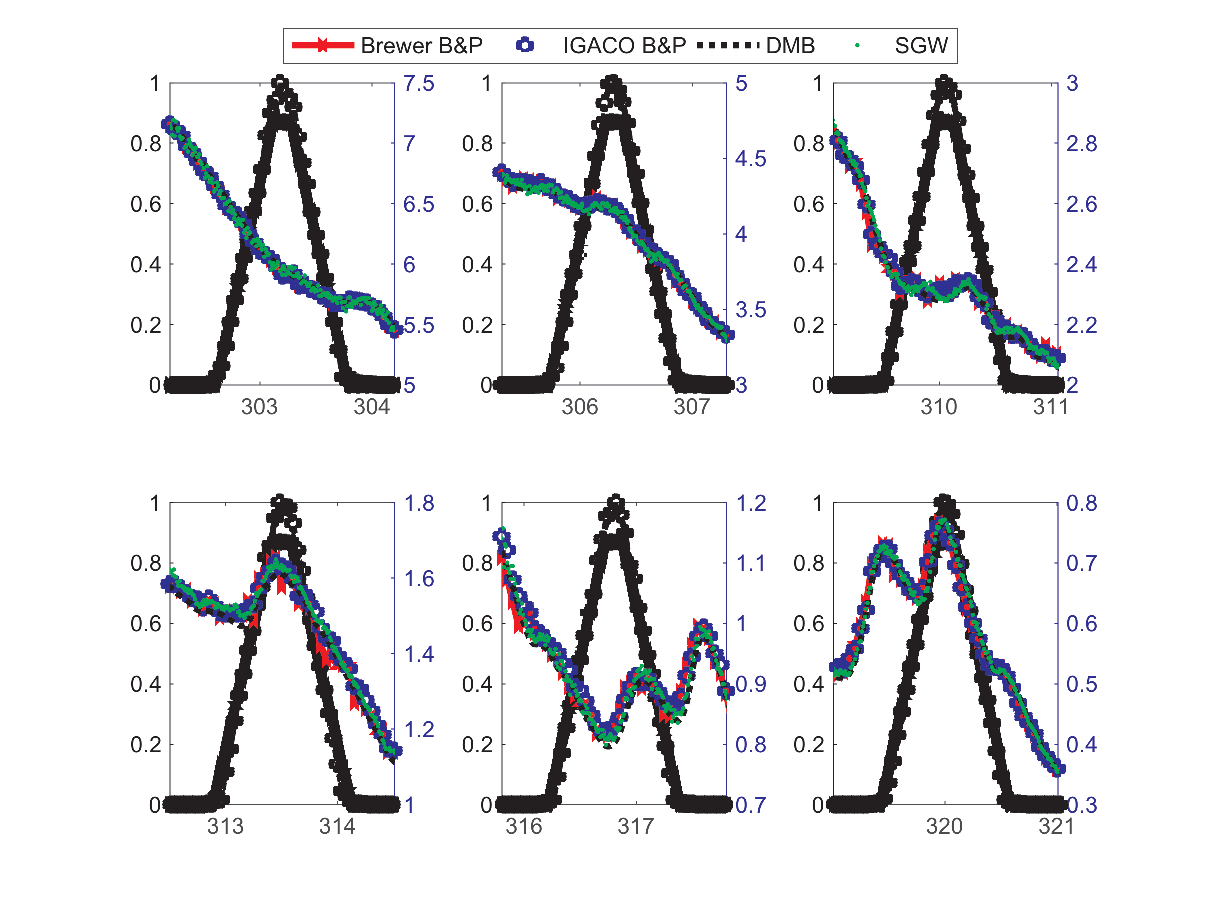
\includegraphics[width=8.3cm]{figures/General_Laser_Brewer_ozone_mode.eps}
\caption{ Plot of the parametrized (thick lines, lext axis) and the measured slit functions (dots, lext axis) as well as the different ozone cross sections (right axis) used for the Brewer effective ozone absorption coefficient calculation.}
\label{fig:param}
\end{figure}

\clearpage
%
\begin{figure}[t]
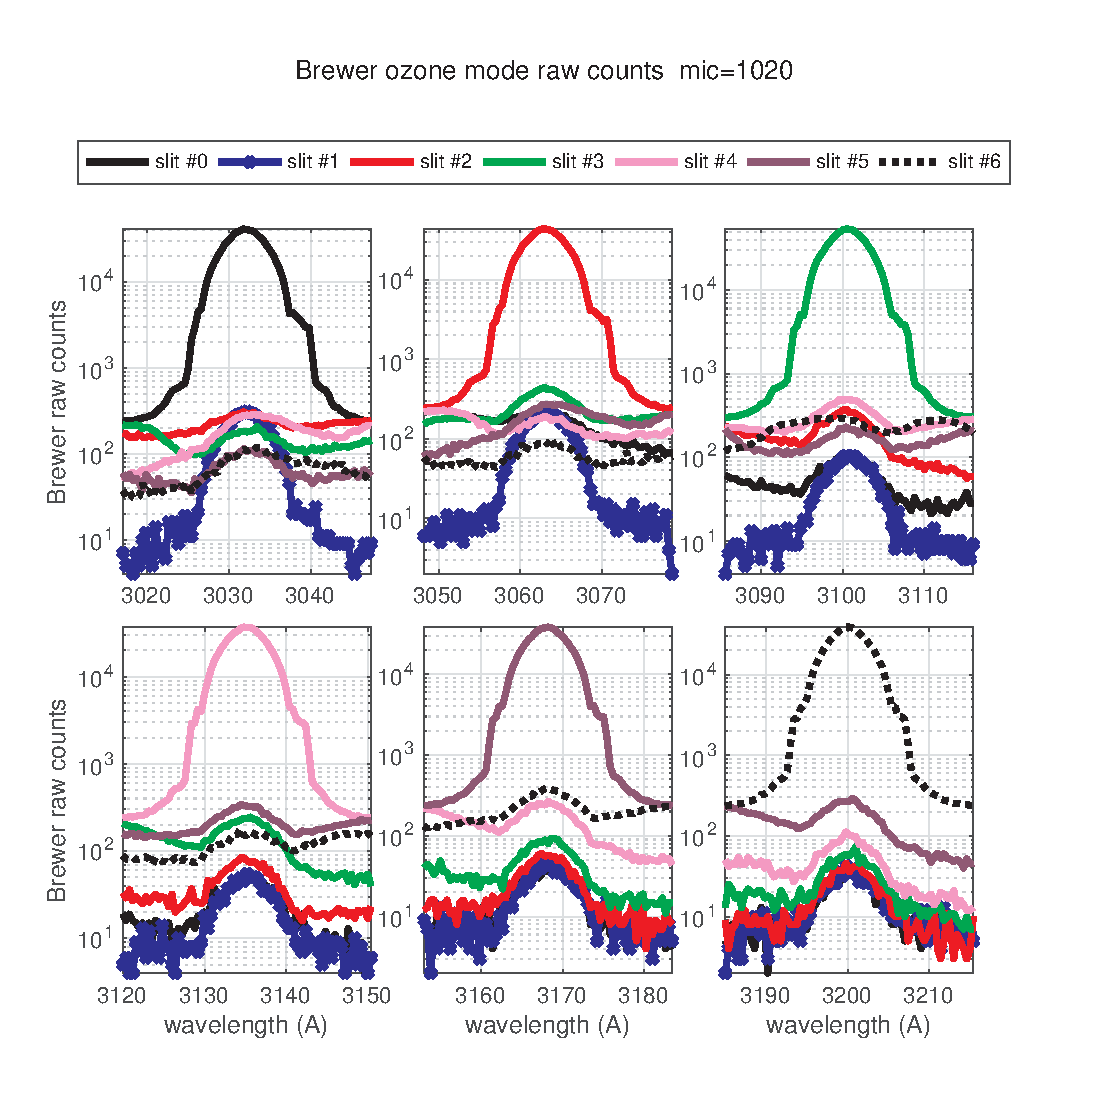
\includegraphics[width=8.3cm]{figures/General_laser_log.eps}
\caption{Brewer measurements in the ozone mode while the laser wavelength is changed every 0.1 nm . The blue curve corresponds to the dark counts obtained from the measurements of slit 1.}
\label{fig:laser_log}
\end{figure}

%
\clearpage
\begin{figure}[t]
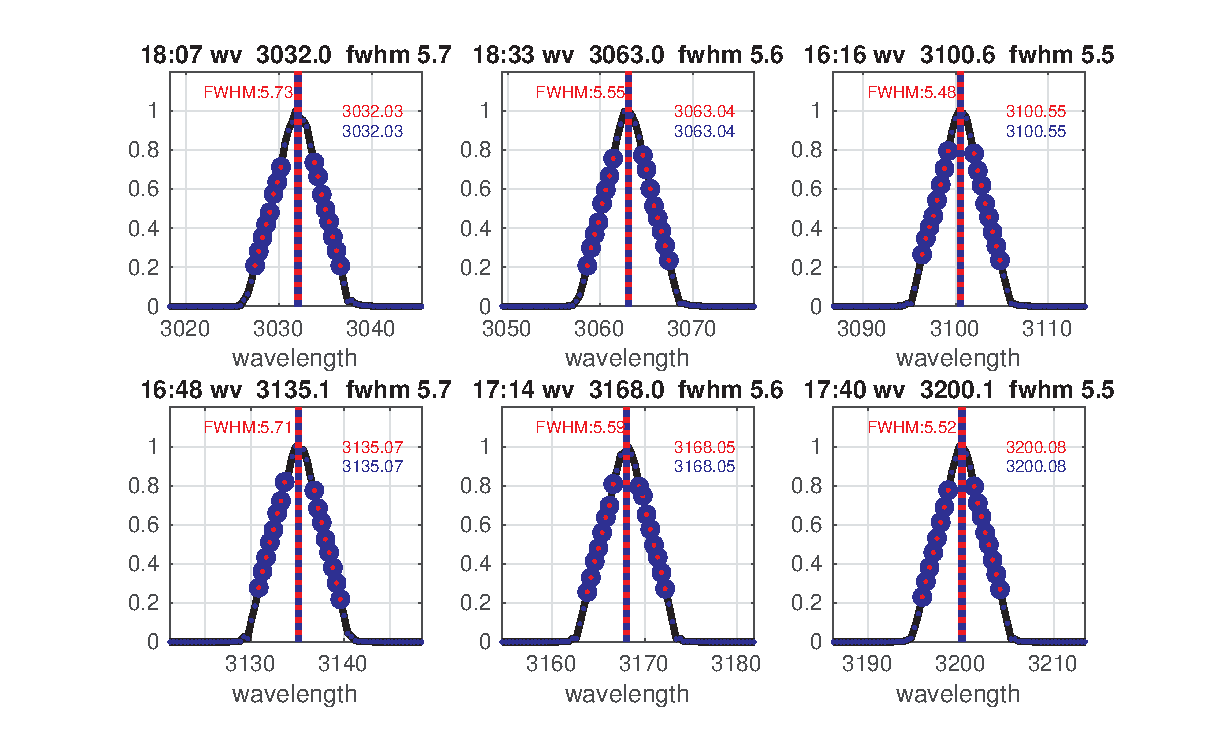
\includegraphics[width=8.3cm]{figures/General_Laser_scan_dsp.eps}
\caption{Brewer measurements in the ozone mode while the laser wavelength is changed every 0.1 nm . The blue curve corresponds to the dark counts obtained from the measurements of slit 1.}
\label{fig:laser_dsp}
\end{figure}


\clearpage
\begin{figure}[t]
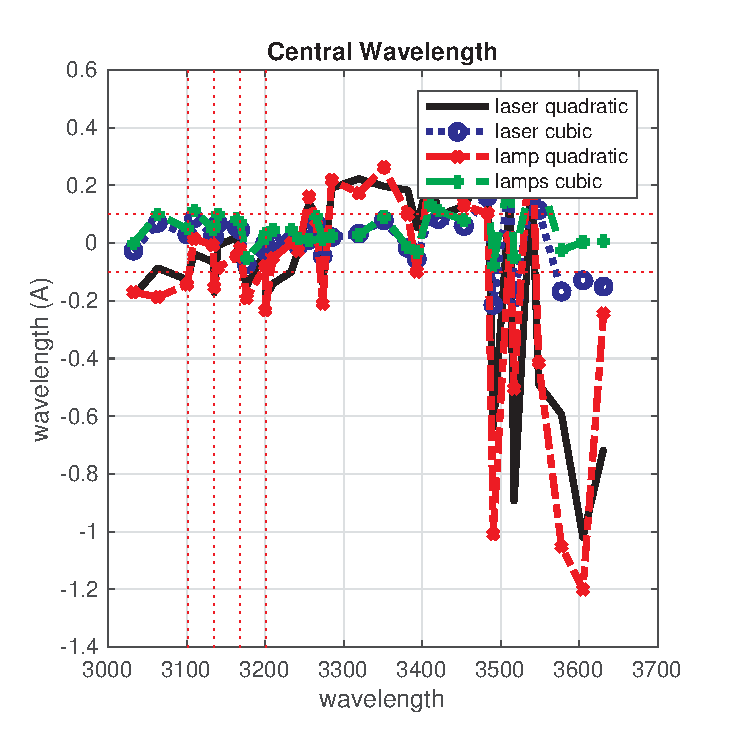
\includegraphics[width=8.3cm]{figures/General_central_comparison.eps}
\caption{Differences between the central wavelengths determinated directly and by the scanning methods: with the laser wavelengths in equally spaced grid every 5nm and lines of the discharge lamps; in both cases quadratic and cubic fitting are used.}
\label{fig:cw_comp}
\end{figure}


 \clearpage
\begin{figure}[t]
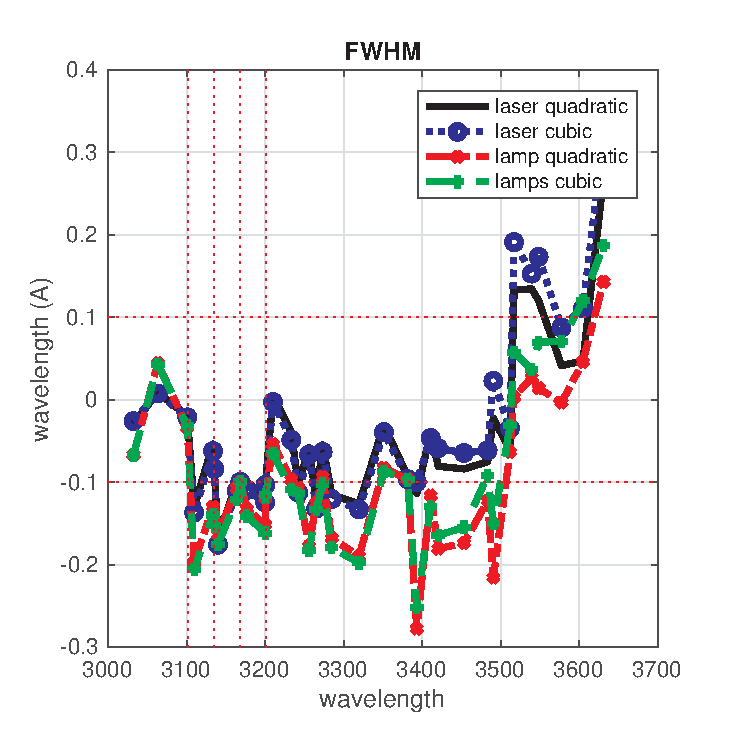
\includegraphics[width=8.3cm]{figures/General_fwhm_comparison.eps}
\caption{Differences between the FWHMs determinated directly and by the scanning methods: with the laser wavelengths in equally spaced grid every 5nm and lines of the discharge lamps; in both cases quadratic and cubic fitting are used.}
\label{fig:fwhm_comp}
\end{figure}

\clearpage

\begin{figure}[t]
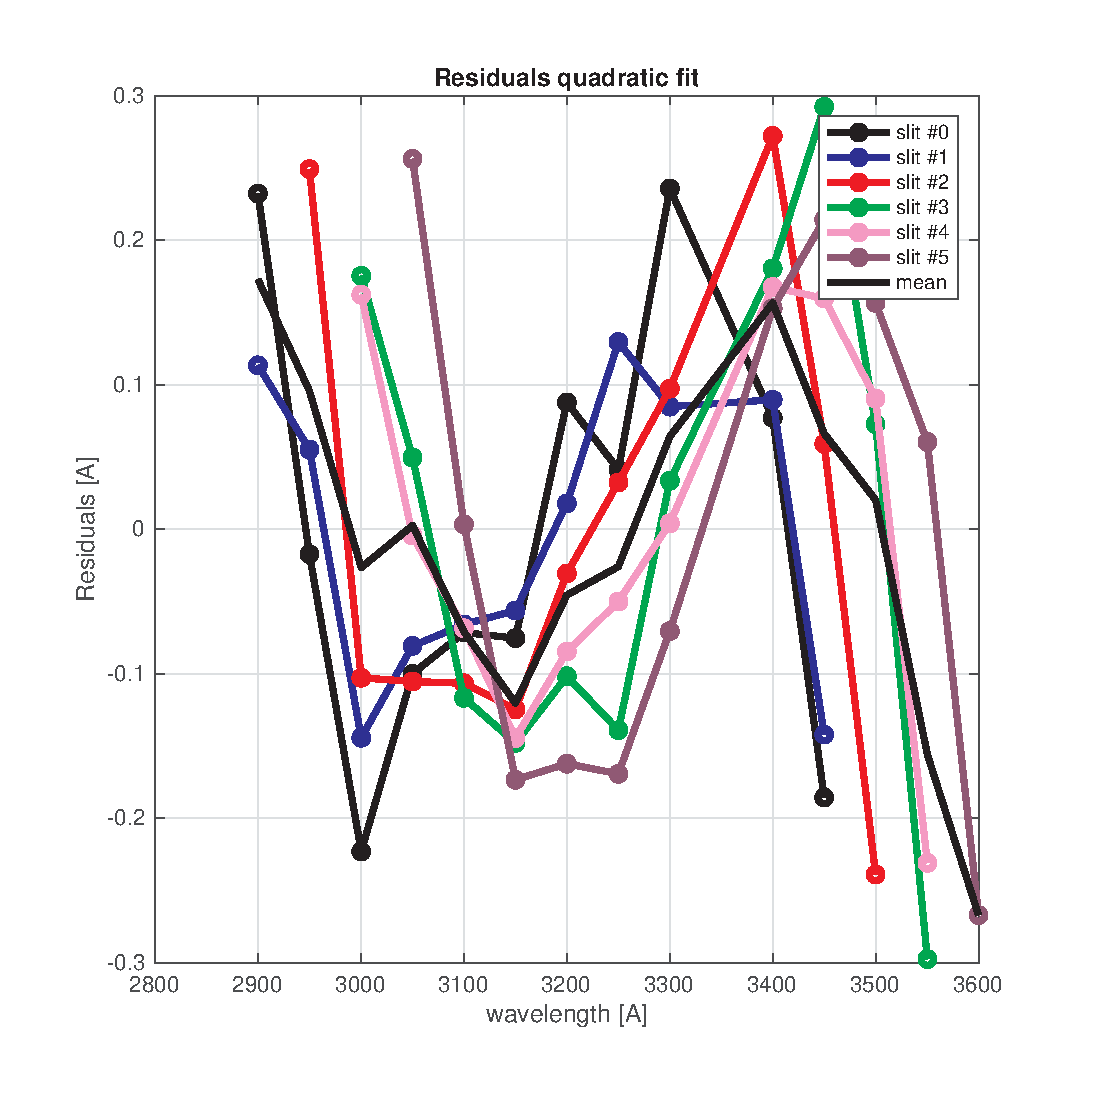
\includegraphics[width=8.3cm]{figures/General_DSP_QUAD_RES.eps}
\caption{ Residuals of the quadratic fit.}
\label{fig:dsp_residual_quad}
\end{figure}

\clearpage
\begin{figure}[t]
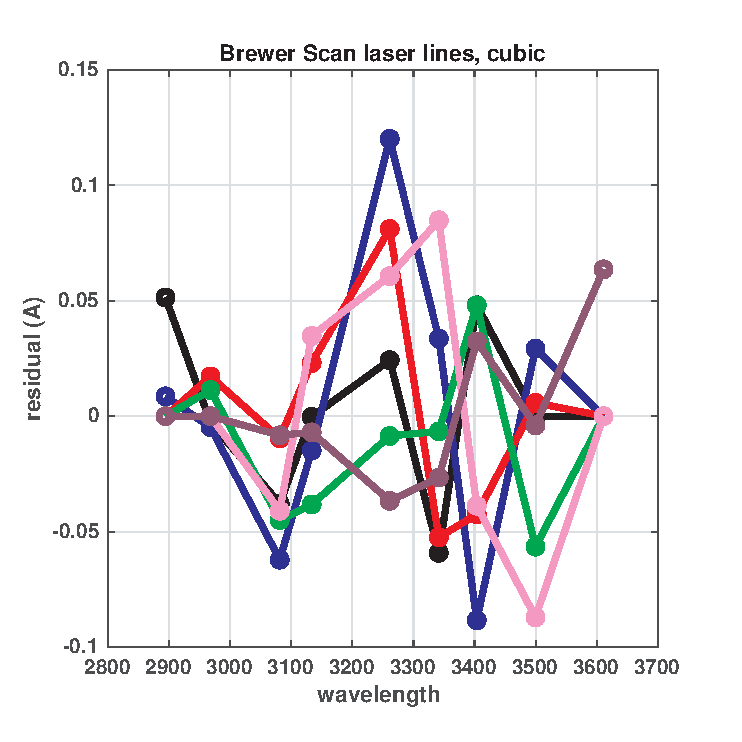
\includegraphics[width=8.3cm]{figures/General_brewer_scan_cubic_residual.eps}
\caption{ Residuals of the cubic fit.}
\label{fig:dsp_residual_cubic}
\end{figure}

%\subsection{HEADING}
%TEXT
%\subsubsection{HEADING}
%TEXT


%\conclusions  %% \conclusions[modified heading if necessary]
%TEXT

%% The following commands are for the statements about the availability of data sets and/or software code corresponding to the manuscript.
%% It is strongly recommended to make use of these sections in case data sets and/or software code have been part of your research the article is based on.

\codeavailability{TEXT} %% use this section when having only software code available


\dataavailability{TEXT} %% use this section when having only data sets available


\codedataavailability{TEXT} %% use this section when having data sets and software code available


%\clearpage

\begin{table}[t]
\caption{Emission lines of the discharge lamps used for Brewer calibration}
\begin{tabular}{lll}
\tophline
Lamp           & Line (nm) & Slits \\
\middlehline
Mercury (Hg)   & 289.36    & 0–1   \\
Hg             & 296.728   & 0–3   \\
Zinc (Zn)      & 301.836   & 0–5   \\
Zn             & 303.578   & 0–5   \\
Cd (multiplet) & 308.082   & 0-5   \\
Cd             & 313.3167  & 0–5   \\
Cd             & 326.1055  & 0–5   \\
Zn             & 328.233   & 0–5   \\
Hg             & 334.148   & 0–5   \\
Cd             & 340.3652  & 0–5   \\
Cd             & 349.995   & 4–5   \\
Cd (multiplet) & 361.163   & 5     \\
\bottomhline
\end{tabular}
\belowtable{} % Table Footnotes
\label{tab:dsp_lines}
\end{table}


%\clearpage

\begin{table}[t]
\caption{Ozone absorption coefficient in atm $cm^-1$ calculated using four absorption cross sections.}
\begin{tabular}{lll}
\tophline
     & Parametrized & Measured \\
\middlehline
BRW  & 0.3381       & 0.3407   \\
B\&P & 0.3330       & 0.3360    \\
DMB  & 0.3483       & 0.3514   \\
SDK  & 0.3392       & 0.3422    \\
\bottomhline
\end{tabular}
\belowtable{} % Table Footnotes
\label{tab:slit_param}
\end{table}


\begin{table*}[t]
\caption{Ozone absorption coefficient in atm $cm^-1$ calculated using  four absorption cross sections (????!!)}
\begin{tabular}{lllllll}
\tophline
     & brw\_scan & ptb\_scan & opo\_quad & opo\_cubic & lamp\_quad & lamp\_cubic \\
\middlehline
SGW   & 0.3409    & 0.3368    & 0.3442    & 0.342      & 0.3446     & 0.3412      \\
ratio & 1         & 0.9881    & 1.0096    & 1.0033     & 1.0108     & 1.001      \\
\bottomhline
\end{tabular}

\belowtable{} % Table Footnotes
\label{tab:o3abs_sum}
\end{table*}


%\appendix
%\section{}    %% Appendix A
%\subsection{}     %% Appendix A1, A2, etc.
%\noappendix       %% use this to mark the end of the appendix section

%% Regarding figures and tables in appendices, the following two options are possible depending on your general handling of figures and tables in the manuscript environment:

%% Option 1: If you sorted all figures and tables into the sections of the text, please also sort the appendix figures and appendix tables into the respective appendix sections.
%% They will be correctly named automatically.

%% Option 2: If you put all figures after the reference list, please insert appendix tables and figures after the normal tables and figures.
%% To rename them correctly to A1, A2, etc., please add the following commands in front of them:

%\appendixfigures  %% needs to be added in front of appendix figures

%\appendixtables   %% needs to be added in front of appendix tables




%% Please add \clearpage between each table and/or figure. Further guidelines on figures and tables can be found below.



%\authorcontribution{TEXT} %% optional section
%\competinginterests{TEXT} %% this section is mandatory even if you declare that no competing interests are present
%\disclaimer{TEXT} %% optional section

\begin{acknowledgements}
This work has been supported by the European Metrology Research Programme (EMRP) within the joint research project ENV59 “Traceability for atmospheric total column ozone” (ATMOZ).  The  EMRP  is jointly funded by the EMRP participating countries within EURAMET and the European Union. 

\end{acknowledgements}




%% REFERENCES

%% The reference list is compiled as follows:

%\begin{thebibliography}{}
%\bibitem[AUTHOR(YEAR)]{LABEL}
%REFERENCE 1
%\bibitem[AUTHOR(YEAR)]{LABEL}
%REFERENCE 2
%\end{thebibliography}

%% Since the Copernicus LaTeX package includes the BibTeX style file copernicus.bst,
%% authors experienced with BibTeX only have to include the following two lines:

 \bibliographystyle{copernicus}
 \bibliography{wv_brewer.bib}
%%
%% URLs and DOIs can be entered in your BibTeX file as:
%%
%% URL = {http://www.xyz.org/~jones/idx_g.htm}
%% DOI = {10.5194/xyz}


%% LITERATURE CITATIONS
%%
%% command                        & example result
%% \citet{jones90}|               & Jones et al. (1990)
%% \citep{jones90}|               & (Jones et al., 1990)
%% \citep{jones90,jones93}|       & (Jones et al., 1990, 1993)
%% \citep[p.~32]{jones90}|        & (Jones et al., 1990, p.~32)
%% \citep[e.g.,][]{jones90}|      & (e.g., Jones et al., 1990)
%% \citep[e.g.,][p.~32]{jones90}| & (e.g., Jones et al., 1990, p.~32)
%% \citeauthor{jones90}|          & Jones et al.
%% \citeyear{jones90}|            & 1990



%% FIGURES

%% When figures and tables are placed at the end of the MS (article in one-column style), please add \clearpage
%% between bibliography and first table and/or figure as well as between each table and/or figure.


%% ONE-COLUMN FIGURES

%%f
%\begin{figure}[t]
%\includegraphics[width=8.3cm]{FILE NAME}
%\caption{TEXT}
%\end{figure}
%
%%% TWO-COLUMN FIGURES
%
%%f
%\begin{figure*}[t]
%\includegraphics[width=12cm]{FILE NAME}
%\caption{TEXT}
%\end{figure*}
%
%
%%% TABLES
%%%
%%% The different columns must be seperated with a & command and should
%%% end with \\ to identify the column brake.
%
%%% ONE-COLUMN TABLE
%
%%t
%\begin{table}[t]
%\caption{TEXT}
%\begin{tabular}{column = lcr}
%\tophline
%
%\middlehline
%
%\bottomhline
%\end{tabular}
%\belowtable{} % Table Footnotes
%\end{table}
%
%%% TWO-COLUMN TABLE
%
%%t
%\begin{table*}[t]
%\caption{TEXT}
%\begin{tabular}{column = lcr}
%\tophline
%
%\middlehline
%
%\bottomhline
%\end{tabular}
%\belowtable{} % Table Footnotes
%\end{table*}
%
%
%%% MATHEMATICAL EXPRESSIONS
%
%%% All papers typeset by Copernicus Publications follow the math typesetting regulations
%%% given by the IUPAC Green Book (IUPAC: Quantities, Units and Symbols in Physical Chemistry,
%%% 2nd Edn., Blackwell Science, available at: http://old.iupac.org/publications/books/gbook/green_book_2ed.pdf, 1993).
%%%
%%% Physical quantities/variables are typeset in italic font (t for time, T for Temperature)
%%% Indices which are not defined are typeset in italic font (x, y, z, a, b, c)
%%% Items/objects which are defined are typeset in roman font (Car A, Car B)
%%% Descriptions/specifications which are defined by itself are typeset in roman font (abs, rel, ref, tot, net, ice)
%%% Abbreviations from 2 letters are typeset in roman font (RH, LAI)
%%% Vectors are identified in bold italic font using \vec{x}
%%% Matrices are identified in bold roman font
%%% Multiplication signs are typeset using the LaTeX commands \times (for vector products, grids, and exponential notations) or \cdot
%%% The character * should not be applied as mutliplication sign
%
%
%%% EQUATIONS
%
%%% Single-row equation
%
%\begin{equation}
%
%\end{equation}
%
%%% Multiline equation
%
%\begin{align}
%& 3 + 5 = 8\\
%& 3 + 5 = 8\\
%& 3 + 5 = 8
%\end{align}
%
%
%%% MATRICES
%
%\begin{matrix}
%x & y & z\\
%x & y & z\\
%x & y & z\\
%\end{matrix}
%
%
%%% ALGORITHM
%
%\begin{algorithm}
%\caption{�}
%\label{a1}
%\begin{algorithmic}
%�
%\end{algorithmic}
%\end{algorithm}
%
%
%%% CHEMICAL FORMULAS AND REACTIONS
%
%%% For formulas embedded in the text, please use \chem{}
%
%%% The reaction environment creates labels including the letter R, i.e. (R1), (R2), etc.
%
%\begin{reaction}
%%% \rightarrow should be used for normal (one-way) chemical reactions
%%% \rightleftharpoons should be used for equilibria
%%% \leftrightarrow should be used for resonance structures
%\end{reaction}
%
%
%%% PHYSICAL UNITS
%%%
%%% Please use \unit{} and apply the exponential notation


\end{document}
